%!TEX program = xelatex
\documentclass[11pt,class=book]{standalone}
%\usepackage[utf8]{inputenc}
\usepackage{fontenc}
\usepackage[table,svgnames]{xcolor}

\usepackage{pgf}
\usepackage{tikz}

\usepackage{array}
\usepackage{tabularx}
\usepackage{multirow}

\usetikzlibrary{shapes}
\usetikzlibrary{arrows.meta}
\usetikzlibrary{calc}

\definecolor{bg_color}{RGB}{250,250,229}

\colorlet{color1}{cyan!50}
\colorlet{color2}{red!30!green!40}
\colorlet{color3}{orange!50}
\colorlet{color4}{violet!60!blue!55}

\newganttlinktype{bartobardown}{
	\ganttsetstartanchor{south east}
	\ganttsetendanchor{north west}
	\draw [/pgfgantt/link] (\xLeft, \yUpper) -- (\xRight, \yLower);
}
\newganttlinktype{bartobarup}{
	\ganttsetstartanchor{north east}
	\ganttsetendanchor{south west}
	\draw [/pgfgantt/link] (\xLeft, \yUpper) -- (\xRight, \yLower);
}
\newganttlinktype{milestonetobardown}{
	\ganttsetstartanchor{south}
	\ganttsetendanchor{north west}
	\draw [/pgfgantt/link] (\xLeft, \yUpper) -- (\xRight, \yLower);
}
\newganttlinktype{bartomilestonedown}{
	\ganttsetstartanchor{south east}
	\ganttsetendanchor{north}
	\draw [/pgfgantt/link] (\xLeft, \yUpper) -- (\xRight, \yLower);
}


\begin{document}
	\pgfmathsetmacro\commitsep{20}%
	\pgfmathsetmacro\diffyshift{25}%

	\begin{tikzpicture}[x=1pt,y=1pt,>=Latex]
		\tikzset{
			commit/.style={
				draw,
				circle,
				fill=white,
				inner sep=0pt,
				minimum size=12pt
			},
			commitname/.style={
				font=\small\tt
			},
			committxt/.style={
				font=\small\tt,
				anchor=west
			},
			diff/.style={
				draw,
				rectangle,
				text width=200,
				inner sep=0.8,
				fill=white
			},
			every path/.style={
				draw
			}
		}

		%---------------------------------
		% Git tree
		\node[commit,green,fill=green] (c1) at (0,0) {};
		\node[commitname] (c1txt) at (c1) {A};

		\node[commit,green,fill=green] (c2) at ($(c1)+(0,\commitsep)$) {};
		\node[commitname] (c2txt) at (c2) {B};
		\path[green] (c1) to[out=90,in=-90] (c2);

		\node[commit,green,fill=green] (c3) at ($(c2)+(0,\commitsep)$) {};
		\node[commitname] (c3txt) at (c3) {C};
		\path[green] (c2) to[out=90,in=-90] (c3);

		\node[commit,green,fill=green] (c4) at ($(c3)+(0,\commitsep)$) {};
		\node[commitname] (c4txt) at (c4) {D};
		\path[green] (c3) to[out=90,in=-90] (c4);

		%---------------------------------
		% M
		\node[commit,red,fill=red] (c5) at ($(c4)+(0,2*\commitsep)$) {};
		\node[commitname] (c5txt) at (c5) {M};
		\path[green] (c4) to[out=90,in=-90] (c5);

		%---------------------------------
		% E
		\node[commit,green!50!blue,fill=green!50!blue] (c6) at ($(c4)+(\commitsep,\commitsep)$) {};
		\node[commitname] (c6txt) at (c6) {E};
		\path[green] (c4) to[out=90,in=-90] (c6);

		\node[
			font=\small\tt,
			gray,
			above,
			anchor=south
		] (master) at (c6.north) {master};

		%---------------------------------
		% M diff
		\node[
			diff,
			anchor=west
		] (img) at ($(c5.east)+(30+\commitsep,\diffyshift)$) {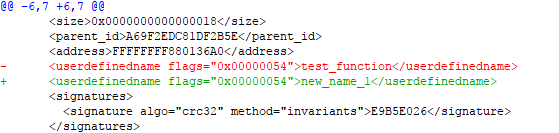
\includegraphics[width=\textwidth]{YaCo_git_diff1}};

		\draw (c5.east) -- ++(\diffyshift,\diffyshift) -- (img.west);

		%---------------------------------
		% E diff
		\node[
			diff,
			anchor=west
		] (img) at ($(c6.east)+(30,-\diffyshift)$) {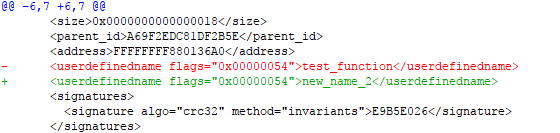
\includegraphics[width=\textwidth]{YaCo_git_diff2}};

		\draw (c6.east) -- ++(\diffyshift,-\diffyshift) -- (img.west);

		%---------------------------------
		% Fetch
		\draw[<-,ultra thick,green] ($(c1)+(0,120)$) -- ++(0,25) node[above] {\footnotesize fetch};
	\end{tikzpicture}
\end{document}
